\section{Slither.io Game}

Slither.io is a multiplayer online video game released in 2016 for iOS, Android, and for web browsers on the website \href{https://Slither.io}{Slither.io}. The game is developed by Steve Howse. Shortly after its releases, the iOS version became the most downloaded app on the App Store, and the browser version was the 250th most visited website worldwide \cite{web:Slitherio_Wikipedia}. This thesis focuses on the the browser version. In the following chapter the game basics are explained, although Slither is more easily understood by \href{https://Slither.io}{playing the game} or to watch a 2 minute \href{https://www.youtube.com/watch?v=cHDrFwX9ROE}{YouTube video} of the gameplay.

\begin{figure}[H]
    \centering
    \href{https://www.youtube.com/watch?v=cHDrFwX9ROE}{
        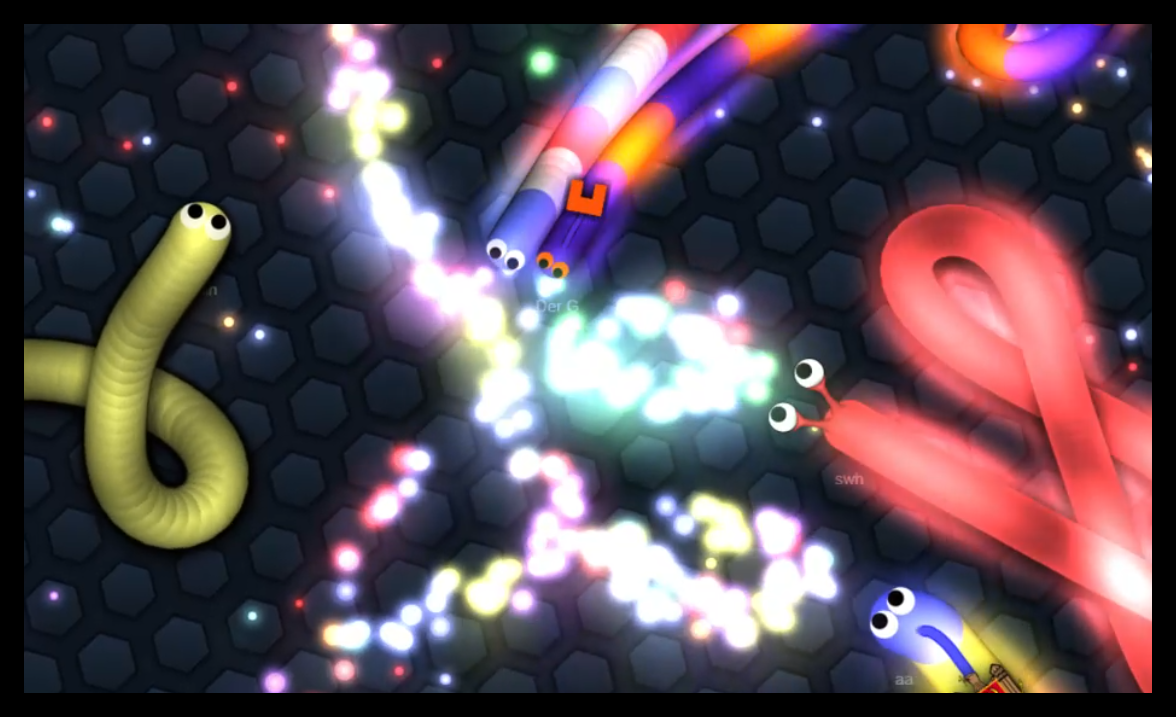
\includegraphics[width=0.75\textwidth]{Figures/Gameplay/Thumbnail Gameplay 3.png}}
    \caption{\centering A screenshot of the gameplay video. The snakes are competing for leftover food pellets of a defeated snake.}
    \label{fig:slitherio_youtube_gameplay}
\end{figure}


\subsection{Game Basics}

Slither.io is a free-for-all online browser game. Free-for-all means that every player competes against each other under the same circumstances. If a player dies it is game-over and the player has to start all over again. The player controls a snake with the mouse or keyboard. The snake is controlled via a left and right direction and a speed boost. The snake dies by colliding into other snakes or hitting the border of the arena. There are hundreds of competing snakes played by people online. The player needs to defeat the other snakes and eat food pellets to reach the goal of being the largest snake in the arena. 
\\\\
The visual aspects of Slither make the game instantly recognisable. Each player can choose the skin of its snake. The snakes consist of multiple connected circles, where the first circle is its googly eyed head. The background of the arena consists of hexagon tiles, and the area outside the arena is dark red. It is best to adjust the browser to a square screen to maximize the viewing area. The heads-up display (HUD) contains information on the state of the game. This includes the player's score and leaderboard rank, the scores of the ten largest snakes, and a map with the locations of the snakes. 
\newpage \noindent
There are four different types of food pellets. Each of these pellets spawns in a different situation and has a specific score value. \textit{Natural} pellets randomly spawn around the arena near players and are worth around 2 points. \textit{Special} pellets are rarer than natural pellets and move away from snakes. These are worth 50 points. The boosting action makes a snake faster, but consumes points. A fraction of these points are converted to \textit{boost} pellets that appear behind the boosting player, worth around 1 point. When a snake dies it drops multiple \textit{death} pellets of around 10 points. When a snake eats pellets, its score increases. The snake gets both longer and wider. Larger snakes have a larger viewing area, but also a larger turning angle.









\subsection{Strategies}
Slither's most popular strategies are discussed in this section. Hopefully, the intelligent agent will be able to learns these strategies through only self-learning. The \href{https://slitherio-archive.fandom.com/wiki/Strategies}{Slither.io Fandom WiKi} contains a list of basic offensive and defensive Slither strategies \cite{web:Slitherio_Community}. The upcoming strategies are based on this list.

\subsubsection*{Offense}
The most basic offensive strategy is to \textit{cut-off} snakes. This is done by suddenly turning in front of another snake while using the speed boost. It is wiser to use this strategy as a smaller snake, since less progress is lost when the cut-off backfires. Meanwhile, it is better to cut-off larger snakes, since larger snakes drop more pellets. Also, cutting off larger snakes can be easier, since they have a larger angle of rotation. However, larger snakes are on average better at the game, so they usually anticipate any cut-off attempt.

\textit{Coiling} is another commonly used offensive strategy. In this strategy, a snake completely surrounds other snakes with its tail. As the snake's coil tightens, the trapped snakes bump into the coil and die. The coiling snake can then eat the dropped pellets. Coiling can be countered by cutting-off the coiling snake at the right time, or by carefully tracing the edges of the coiled region until the coiling snake gives up. Coiling is also not without risk, because a coiling snake is more predictable, and can be coiled itself more easily. A more advance technique of coiling is to bait snakes with leftover candy and to trap them inside a coil.

\subsubsection*{Defense}

A snake can protect itself against dangerous situations by boosting away to less crowded areas, or by making use of its tail. The tail can be used as a shield to defense against other snake, and as a safe return path. If a snake is passing through two snakes, the middle snake is sometimes \textit{wedged} in between the outer snakes. A snake should always be able to turn around, to avoid a potential wedge. 

Players don't have to defeat other snakes to eat dropped pellets. It is often safer and just as profitable to let other snakes defeat each other and dive in at the right time to steal the pellets. A specific scavenging technique is to follow a snake in the hopes it dies. A snake is more likely to die in boost mode, since boosting makes is harder to control the snake, and snakes boost more frequently in crowded and dangerous situations. So large boosting snakes are the best snakes to follow. 



